%%%%%%%%%%%%%%%%%%%%%%%%%%%%%%%%%%%%%%%%%%%%%%%%%%%
%
%  New template code for TAMU Theses and Dissertations starting Fall 2012.  
%  For more info about this template or the 
%  TAMU LaTeX User's Group, see http://www.howdy.me/.
%
%  Author: Wendy Lynn Turner 
%	 Version 1.0 
%  Last updated 8/5/2012
%
%%%%%%%%%%%%%%%%%%%%%%%%%%%%%%%%%%%%%%%%%%%%%%%%%%%
%%%%%%%%%%%%%%%%%%%%%%%%%%%%%%%%%%%%%%%%%%%%%%%%%%%%%%%%%%%%%%%%%%%%%%
%%                           SECTION III
%%%%%%%%%%%%%%%%%%%%%%%%%%%%%%%%%%%%%%%%%%%%%%%%%%%%%%%%%%%%%%%%%%%%%



\chapter{\uppercase{Targeted Observations with the VIRUS Prototype Instrument}}

\section{INTRODUCTION} Clusters of galaxies form the largest bound objects in the universe, and as such their study is a cornerstone in modern day astronomy. Thought to form out of the primordial density fluctuations in the very early universe, the number and distribution of galaxy clusters across the sky is the finger print of the cosmology imprinted on the universe at its birth. The $\Lambda$CDM model of cosmology makes explicit predictions about the number and masses of galaxy clusters throughout the universe. Connecting these predictions to a set of, sufficiently large in size, observed clusters remains a principal problem. Specifically, the largest threat to modern, precision, cluster cosmology is not the identification of large numbers of clusters (the total number of clusters known is only going up) but the accurate recovery of galaxy cluster mass \citeeg{Sehgal2011,Plank2014, Bocquet2015}. 

As mass is not a direct observable, a lot of work is underway to characterize galaxy cluster masses with an observable feature of galaxy clusters. Observed X-ray temperatures and luminosities correlate tightly with a cluster's dynamical mass \citeeg{Mantz2010, Rykoff2014}, especially for dynamically relaxed clusters \citeeg{Mantz2015}. The Sunyaev--Zel'dovich effect (SZE; \citealt{Sunyaev1972}), which uses the up--scattering of cosmic microwave background (CMB) photons to estimate cluster masses, provides accurate estimations of mass \citeeg{Vanderlinde2010, Sehgal2011}, but the ability to detect low mass galaxy clusters is currently limited by technology \citeeg{Carlstrom2002a}. Optical studies \citeeg{Rozo2010, Rozo2015a} primarily use the richness \citeeg{Abell1958,Rykoff2012} or galaxy velocity dispersions to estimate the mass, and are often used to calibrate other mass estimators \citeeg{Ruel2014, Sifon2015}. 

Today, the greatest number of clusters are being discovered using large SZE surveys with the South Pole Telescope (SPT; \citealt{Carlstrom2011}) or the Atacama Cosmology Telescope (ACT; \citealt{Swetz2011}). However, deep, wide field optical surveys, such as the Dark Energy Survey (DES; \citealt{DES2005}) will discover many more, low mass clusters in the near future. Such clusters will rely on spectroscopic follow up to better constrain their dynamical mass. But, as the number of clusters grows to many tens of thousands, spectroscopic followup becomes unfeasible. Therefore, large, single telescope, spectroscopic surveys will be required to reduce systematics and calibrate the observable--mass relation to a level that will allow accurate mass estimations using other methods.

In this work, we present a pilot study of ten massive galaxy clusters using integral field spectroscopy with the Mitchell Spectrograph as a pilot program for the Hobby Eberly Dark Energy Experiment (HETDEX; \citealt{Hill2008}) survey. HETDEX is a forthcoming blind spectroscopic survey that could potentially be used to accurately calibrate the observable--mass relation for a significant number of galaxy clusters at both extremes of the mass scale. At present, because HETDEX is designed to measure the dark energy equation of state at $z\sim2$, the applicability to galaxy cluster science has not yet been investigated. We began this investigation with \defcitealias{Boada2016}{Paper I}\cite{Boada2016} (hereafter \citetalias{Boada2016}). The second installment of this two part work, the goal of this study is to obtain spectroscopic redshifts of the individual cluster galaxies, determine the velocity dispersion and to infer each cluster's dynamical mass. This allows us to compare the inferred mass with other mass estimators (\eg, the clusters in this sample have deep \textit{Chandra} or \textit{XMM-Newton} X-ray data, and richness measurements) with the aim of reducing the scatter in the richness--mass relation, $\sigma_{M|\lambda}$. The ability of HETDEX to further constrain optically derived masses is of paramount importance to upcoming large photometric surveys. This study provides insight into how well a HETDEX type survey will constrain mass estimations and cosmological parameters in the future.

The layout of this work is the following. In Section~\ref{sec:design} we discuss the target selection and the setup of the MS used to conduct the observations. Section~\ref{sec:data reduction} describes the methods and tools used to reduce the observations. We present our redshift catalog, cluster members and cluster dynamical properties in Section~\ref{sec:analysis}. In Section~\ref{sec:discussion}, we compare and discuss the different mass estimations and remark on the applicability of these methods for HETDEX. Finally, we summarize this work in Section~\ref{sec:summary}.

Throughout this paper, we use a concordance cosmological model ($\Omega_\Lambda = 0.7$, $\Omega_m = 0.3$, and $H_0= 70$ \kms \mpc), assume a Chabrier initial mass function \citep{Chabrier2003}, and use AB magnitudes \citep{Oke1974} unless specifically noted.

\section{DESIGN}\label{sec:design} 
\subsection{Target Selection}\label{sec:selection} We select clusters at $z=0.2-0.3$ using two different methods and for two different purposes. Eight of the ten clusters are optically selected from \cite{Rykoff2012} using the \textit{Sloan Digital Sky Survey} (SDSS; \citealt{Blanton2001a}) Data Release 8. These clusters have high ($M_{DM} > 8\times10^{14}\msol$) optically traced mass (richness; discussed further below). The last two clusters are selected from the \textit{XMM Cluster Survey} (XCS; \citealt{Mehrtens2012}) and correspond to individually measured X-ray temperatures of $T_X < 2.5$ keV. Such X-ray temperatures have inferred masses of $10^{14}\msol > M_{DM} > 5\times10^{13}\Msol$.

The optically selected clusters have many more members (see Table~\ref{tbl: derived parameters}) than the X-ray selected clusters which allows us to investigate the accuracy of our mass recovery methods at both cluster and group scales. See Table~\ref{tbl:targets} for individual cluster sky positions and associated parameters. 
\begin{table*}
	\caption{Galaxy clusters targeted with the MS: Cluster is our local name; $z$ is the nominal (often photometric) redshift of the cluster.} 
	\begin{tabular}
		{lccccccc} \hline Cluster & Alt. Name & RA (J2000) & DEC (J2000) & $z$ \\
		\hline \hline
		c16p23+0p06 & SOGRAS J0104+0003 & 01:04:55.369 & +00:03:36.28 & 0.277 & \\
		c203p83+41p0 & Abell 1763 & 13:35:20.092 & +41:00:04.12 & 0.223 \\
		c210p2+02p8 & Abell 1835 & 14:01:01.965 & +02:52:42.63 & 0.252 & \\
		c234p2+24p4 & MaxBCG J234.23439+24.40877 & 15:36:56.253 & +24:24:31.60 & 0.226 & \\ 
		c250p08+46p7 & Abell 2219 & 16:40:19.812 & +46:42:41.51 & 0.225 \\
		c260p61+32p13 & Abell 2261 & 17:22:27.182 & +32:07:57.24 & 0.224 \\
		c319p70+0p56 & MaxBCG J319.70446+00.56035 & 21:18:49.069 & +00:33:37.33 & 0.270 \\
		c328p33+0p19 & Abell 2392 & 21:54:22.936 & +00:37:23.48 & 0.223 \\
		XMMXCSJ124425.9+164758.0 & WHL J124425.4+164756 & 12:44:25.203 & +16:47:48.00 & 0.235 \\
		XMMXCSJ125650.2+254803.2 & \nd & 12:56:49.999 & +25:48:02.99 & 0.280 \\
		\hline 
	\end{tabular}
	\label{tbl:targets} 
\end{table*}

\subsection{The Mitchell Spectrograph} The Mitchell Spectrograph (MS; formerly known as VIRUS-P; \citealt{Hill2008a}) is an integral field unit (IFU) in a square array of 246 $4.24''$ diameter optical fibers. This provides a $1.7'~\times~1.7'$ field-of-view (FOV) with a 1/3 filling factor. A Fairchild Instruments, 2k$\times$2k charge couple device (CCD) images the spectra from each of the 246 fibers. The spectra have approximately a gaussian profile with a 5 pixel full width at half maximum (FWHM), and each are separated by 8 pixels to minimize the amount of cross-talk between the fibers. 

There are two spectral configurations available on The Mitchell Spectrograph, a blue setup, 3600-5800 \AA\ and a red setup, 4600-6800 \AA. In addition, there are four volume phase holographic gratings available to disperse the light. For the purpose of this work, the lowest resolution, $\sim5$\AA, grating is used. Using $1\times1$ binning, this translates into a spectral dispersion of $\sim1.11$ \AA\ pixel$^{-1}$. 

\subsection{Observations} 
\begin{figure}
	\includegraphics[width=\textwidth]{./figures/pointing.eps} \caption{SDSS r-band image of an optically selected galaxy cluster selected from the SDSS DR8 data. The field is centered on the BCG, which has a measured spectroscopic redshift from SDSS of $z = 0.277$. The large black circle shows the region $R<0.5$ Mpc ($r<2.3'$). Nearly all galaxies within this region are associated with the cluster. The four MS fields (and fiber positions for the first dither position) are overdrawn on the field, illustrating how we survey each cluster.} \label{fig:tiles} 
\end{figure}

We use the Mitchell Spectrograph to target the galaxy clusters using the 5\AA\ grating covering a wavelength range of 4400 - 6600\AA. With this instrumental setup and for galaxies $z = 0.2-0.3$, we will cover the Ca H\&K, Fe I ($\lambda 4383$), H-$\delta$, H-$\gamma$ and H-$\beta$ absorption features. Additionally, we cover emission of the [O II] ($\lambda\lambda 3727-3729\AAA$) doublet, H-$\beta$, and [O III] ($\lambda\lambda4960,5008$), which allows for the identification of actively star-forming galaxies.

The FOV of the MS corresponds to an approximately 0.4 Mpc square region at $z = 0.2-0.3$. To ensure adequate coverage of the cluster out to 0.5 Mpc, we use four MS pointings per cluster. Figure~\ref{fig:tiles} shows an example of the tiling done on each cluster. The northeast, northwest, southwest, and southeast fields with the fiber positions are shown in black, blue, green and purple respectively. The entire field is centered on the brightest cluster galaxy (BCG) and the individual tiles are shifted away. Furthermore, each of the four tiles are dithered at relative positions $(\Delta \alpha, \Delta \delta)=(0.0'',0.0'')$, $(-3.6'',-2.0'')$, and $(0.0'', -4.0'')$ from the origin to ensure full coverage of the FOV. Therefore, there are 736 individual spectra for each of the four fields or 2952 measurements for the cluster as a whole.

\editorial{Gotta talk to casey about these exposure times. I'm not sure how it all works out.} We have set exposure times to achieve spectra with signal-to-noise ratios (SNRs) $\sim3$ per spectral element in the continuum for objects with g = 21.3 mag (which corresponds to approximately 0.2L* for cluster galaxies at $z = 0.2$). We base the expected SNR on the experience of \cite{Shetrone2010}, who achieves SNR = 100 per pixel in the continuum for point sources with B=16.5 mag at 4000\AA\ in 4800 seconds. Therefore, for our faintest objects with B $\approx$ g = 21.3 mag, we expect to achieve SNR = 3 per spectral element (averaged over 4.6 pixels) in 3600 seconds per pointing. We require 4 pointings to cover the full area for each cluster. Therefore, we require 1 hr/pointing $\times$ 4 pointings = 4 hrs on sky per cluster. Even though the field is dense with galaxies, there is sufficient ``blank'' area to allow for enough ``sky'' fibers for background subtraction. Therefore, no ``sky'' exposures are required. \editorial{The math doesn't quite work out for the exposure times.}

\section{DATA REDUCTION}\label{sec:data reduction} 
All data are reduced using \textsc{p3d} \citep{Sandin2010} a general-use IFU reduction pipeline. The first step is to min/max-filtered average combine a minimum of twenty bias images from each night into a master-bias image, which is subtracted from each other image from the same night. Secondly, a trace mask is created from flat-fielding on the dusk or dawn sky. The fibers are fairly densely packed, so to determine the position of each spectrum in the dispersion direction each spectrum is extracted using a multi-profile deconvolution approach \citep{Sharp2010} to account for cross talk between fibers. Third, a dispersion mask for the wavelength calibration from images of Hg+Cd (for the May, 2012 observations) or Cd+Ne (for all other observations) arc lamps. The residuals between the derived wavelength solution and the known wavelengths of the emission lines is calculated from a fifth order polynomial and lie between. Finally, a fiber flat is created from the sky flats by a min/max-filtered average combine as in step one. 

All that remains is the extraction of the science images, however there are several steps in this process. First, the science frames are bias subtracted. Next each frame is cleaned of cosmic ray hits using the \textsc{PyCosmic} \citep{Husemann2012} integrated into \textsc{p3d} with the default parameters. Third the extracted spectra are wavelength calibrated using the previously created dispersion mask. Any flexure in the instrument between the images of the arc lamps and science frames is accounted for by aligning the dispersion mask to bright telluric lines (namely 5577~\AA). Finally the extracted spectra are normalized using the transmission in the fiber flat from above.

The result of this process is a row-stacked spectrum (RSS) where each of the 246 fibers are stored individually. A table of fiber positions maps each spectrum onto the image plane. However, for many of our observations a precise astrometric solution for the fiber positions is unknown. The position of the individual fibers but be recomputed by observing dense star fields after each telescope service in which the MS is involved. To correct our fiber positions we first identify fibers which observe stars and identify which fibers the astrometric solution indicates should contain stars. In many cases the stars are located between fibers. To account for this we use a simple Gaussian centroid weighted by the observed flux  to find the correct sky position of the star. We then shift the fiber grid to match the sky position of the stars as reported by the SDSS. For each observation we use as many stars as possible and combine the shifts to generate a mean offset. This offset is applied to all dithers of each observation. There is little need to obtain highly accurate fiber positions as the $4.24''$ fibers insures that reasonably correct positions will identify which fibers should and should not contain galaxies.

A simple sky subtraction scheme is used to remove the majority of sky contamination. Because the majority of fibers for any single pointing are empty, we use a $3\sigma$ clipped median selection to identify sky fibers and a simple average to combine them. The result is then subtracted from every fiber. This adequately removes the bulk of sky emission lines, but often fails to completely remove the \ion{O}{i} line at 5577\AA. This line is masked throughout the determination of redshifts.

% \begin{figure}
% 	\centering
% 	\mbox{
% 	\subfigure{\includegraphics[width=\textwidth]{./figures/c203p83+41p0_mosaic.pdf}}\quad
% 	\subfigure{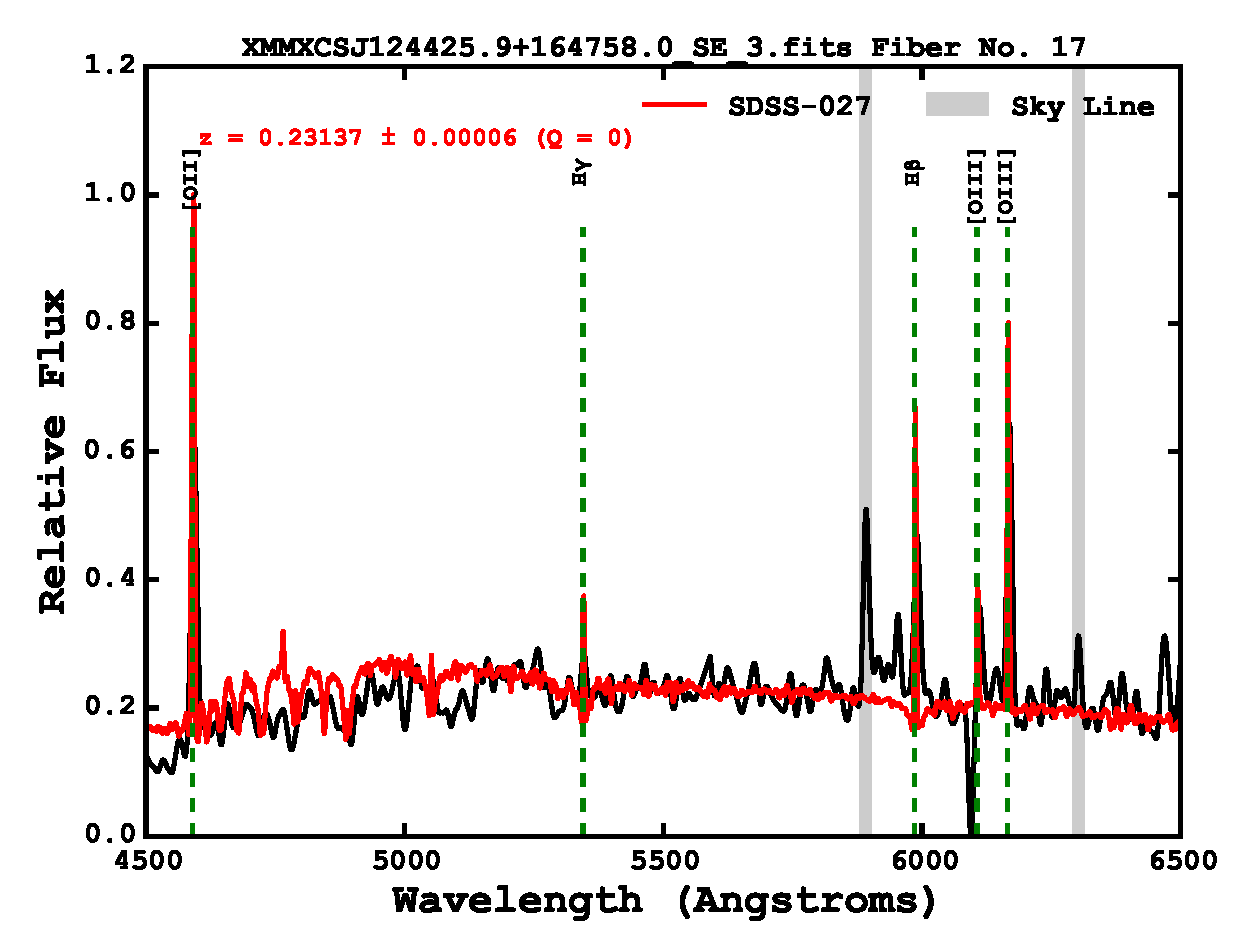
\includegraphics[width=\textwidth]{./figures/spectrum.eps} }}
% 	\caption{SDSS \sdssr\ image of cluster c203p83+41p0. The symbols show the position of observed galaxies. Blue circles indicate galaxies with $Q=0$ or $Q=1$ spectroscopic redshifts, red squares indicate galaxies where a redshift could not be reliably determined, and the orange diamond corresponds to galaxies with pre-existing redshifts from the SDSS. \textit{Right:} Example spectrum of an emission-line cluster galaxy (black line) and template fit (red line) from VIRUS-P on the McDonald 2.7m telescope. The spectrum shows the wavelength range and data quality expected from HETDEX-like spectroscopy, which are sufficient to measure galaxy redshifts.} \label{fig:c203p83+41p0}
% \end{figure}

After reducing all spectra we find an average residual mismatch in the wavelength solution of $\sigma_\lambda \sim 0.4$ \AAA\ or 24 \kms at 5000 \AAA. Fitting gaussians to each of the arc lines we find an average instrumental resolution of $\sim144$ \kms, and combining the two in quadrature gives a total instrumental resolution of $\sigma_{inst} = 146$ \kms, similar to that of other studies using the MS \citeeg{Murphy2011, Blanc2013}.

\section{ANALYSIS}\label{sec:analysis} The analysis of our reduced spectra occurs in two stages. First we derive individual redshifts using the observed galaxies, and then we work with the redshifts collectively to identify which galaxies likely belong to the galaxy cluster in question. This section outlines the steps required in each of those processes. 

Individual galaxy selection is done through cross matching the IFU fiber sky positions with galaxies selected from the SDSS. We select all galaxies brighter than 22 mag in \sdssg\ within $3'$ of the BCG in each cluster. For each galaxy we query the SDSS for photometry in all SDSS bands (\sdssu\sdssg\sdssr\sdssi\sdssz), photometric redshift, and any spectroscopic redshift. 

Because of the large number of fiber pointings, only fibers which overlap with SDSS sources are considered for redshift analysis. Figure \ref{fig:c203p83+41p0} shows cluster c203p83+41p0 with the SDSS detections and measured redshifts overlaid. Orange diamonds are galaxies with SDSS available redshifts. The blue circles and red squares correspond to galaxies where a redshift was and was not determined from the observed spectra. See the appendix for similar figures of the remaining nine clusters.

\subsection{Redshift Catalog}\label{sec:redshift catalog} 
A redshift solution is determined for each galaxy by cross-correlating \citep{Tonry1979} each of the spectra with six galaxy template spectra from the SDSS\footnote{http://classic.sdss.org/dr7/algorithms/spectemplates/index.html} using the \textsc{xcsao} task in the \textsc{iraf} \textsc{rvsao} package \citep{Kurtz1992, Kurtz1998}. For each galaxy we select the spectral template with the highest cross-correlation coefficient and visually inspect the fit. During visual inspection a ``Q'' or quality flag is assigned. High-confidence redshifts, clearly determined by at least two obvious features (such as the Ca H, K and E absorption features), receive $Q=0$, spectra with only a single strong feature (\eg, [\ion{O}{ii}] emission) are assigned $Q=1$ and redshifts resulting from enigmatic features are assigned $Q=2$. For the determination of cluster properties we only consider $Q=0$ and $Q=1$ quality flags. 

\begin{figure}
	\includegraphics[width=\textwidth]{figures/redshiftHist.pdf} 
	\caption{Redshift recovery fractions across all clusters. The bar heights represent the fraction of the total redshifts with the respective $Q$ value at a particular magnitude. For example, $\sim 40\%$ of the $Q=2$ redshifts have $m_r = 20.5-21$. We find a general decrease in redshift quality with increasing $m_r$. } \label{fig:redshiftHist} 
\end{figure}

Figure \ref{fig:redshiftHist} shows the breakdown of $Q$ values for the redshifts across all clusters. We compute 447 redshifts, of which 44\% have $Q=0$, 27\% have $Q=1$ and 29\% have $Q=2$. We find a general decrease in $Q$ flag with increasing $m_r$. Approximately 30\% of the $Q=0$ redshifts correspond to galaxies with $19 < m_r <20$ whereas about 40\% $Q=2$ galaxies have $m_r = 20.5-21$.

\begin{table*}
	\centering \caption{Spectroscopic redshifts for galaxies in C203p8+41p0 measured with the MS: $m_r$ is the observed SDSS \sdssr\ magnitude. $z$ is the derived redshift. $Q$ is the redshift quality flag; see Section~\ref{sec:redshift catalog}. Member? indicates whether the galaxy is a member of the cluster; see Section~\ref{sec:cluster membership}. See the appendix for similar tables for the remaining nine clusters.} 
	\begin{tabular}{ccccccccccc} 
		\hline 
		tile & dither & fiber & ra & dec & r (mag) & redshift & Q & Member & R (Mpc) & LOSV (\kms) \\
		\hline \hline 
		NE & 1 & 14 & 13:35:27.004 & +41:01:36.20 & 20.47 & 0.2019$\pm{0.0003}$ & 1 & ... & 0.40 & -6945$\pm{146}$ \\
		NE & 1 & 111 & 13:35:24.177 & +41:00:54.16 & 20.10 & 0.1178$\pm{0.0001}$ & 1 & ... & 0.15 & -27397$\pm{63}$ \\
		NE & 1 & 154 & 13:35:23.853 & +41:00:33.19 & 19.28 & 0.2214$\pm{0.0002}$ & 0 & ... & 0.18 & -2214$\pm{83}$ \\
		NE & 2 & 6 & 13:35:21.777 & +41:01:34.15 & 20.38 & 0.1691$\pm{0.0002}$ & 1 & ... & 0.27 & -14929$\pm{102}$ \\
		NE & 2 & 14 & 13:35:26.632 & +41:01:33.06 & 20.95 & 0.0403$\pm{0.0003}$ & 0 & ... & 0.09 & -46214$\pm{131}$ \\
		NE & 2 & 63 & 13:35:20.998 & +41:01:08.49 & 17.90 & 0.2381$\pm{0.0001}$ & 0 & $\checkmark$ & 0.25 & 1849$\pm{49}$ \\
		NE & 3 & 22 & 13:35:22.879 & +41:01:24.60 & 19.76 & 0.2386$\pm{0.0003}$ & 0 & $\checkmark$ & 0.33 & 1961$\pm{131}$ \\
		NE & 3 & 25 & 13:35:24.669 & +41:01:26.21 & 19.54 & 0.1444$\pm{0.0001}$ & 0 & ... & 0.25 & -20924$\pm{58}$ \\
		NE & 3 & 73 & 13:35:18.447 & +41:01:00.60 & 19.63 & 0.0779$\pm{0.0001}$ & 0 & ... & 0.09 & -37080$\pm{29}$ \\
		NE & 3 & 106 & 13:35:20.957 & +41:00:50.19 & 18.83 & 0.2235$\pm{0.0002}$ & 0 & $\checkmark$ & 0.17 & -1691$\pm{78}$ \\
		NE & 3 & 147 & 13:35:19.341 & +41:00:31.82 & 19.48 & 0.2380$\pm{0.0001}$ & 0 & ... & 0.11 & 1822$\pm{73}$ \\
		NE & 3 & 185 & 13:35:24.990 & +41:00:18.06 & 20.51 & 0.1887$\pm{0.0002}$ & 1 & ... & 0.18 & -10169$\pm{83}$ \\
		NE & 3 & 206 & 13:35:20.095 & +41:00:04.12 & 16.39 & 0.2274$\pm{0.0001}$ & 1 & $\checkmark$ & 0.00 & -763$\pm{34}$ \\
		NE & 3 & 210 & 13:35:22.528 & +41:00:05.00 & 19.59 & 0.2242$\pm{0.0001}$ & 1 & $\checkmark$ & 0.10 & -1543$\pm{49}$ \\
		NW & 1 & 127 & 13:35:16.384 & +41:00:47.33 & 17.43 & 0.2377$\pm{0.0001}$ & 0 & $\checkmark$ & 0.23 & 1752$\pm{68}$ \\
		NW & 1 & 167 & 13:35:14.400 & +41:00:29.73 & 19.69 & 0.2333$\pm{0.0002}$ & 0 & $\checkmark$ & 0.26 & 690$\pm{117}$ \\
		NW & 2 & 27 & 13:35:17.216 & +41:01:27.25 & 20.21 & 0.1512$\pm{0.0002}$ & 0 & ... & 0.24 & -19279$\pm{117}$ \\
		NW & 2 & 63 & 13:35:12.486 & +41:01:10.57 & 18.84 & 0.1638$\pm{0.0001}$ & 0 & ... & 0.31 & -16210$\pm{44}$ \\
		NW & 2 & 73 & 13:35:09.729 & +41:01:03.49 & 20.00 & 0.2402$\pm{0.0001}$ & 1 & ... & 0.50 & 2367$\pm{58}$ \\
		NW & 2 & 165 & 13:35:12.728 & +41:00:25.16 & 18.74 & 0.2394$\pm{0.0001}$ & 0 & $\checkmark$ & 0.33 & 2155$\pm{58}$ \\
		NW & 2 & 171 & 13:35:16.434 & +41:00:25.31 & 21.68 & 0.1617$\pm{0.0002}$ & 1 & ... & 0.13 & -16728$\pm{121}$ \\
		NW & 2 & 173 & 13:35:17.911 & +41:00:27.16 & 19.49 & 0.1039$\pm{0.0002}$ & 0 & ... & 0.06 & -30763$\pm{107}$ \\
		NW & 2 & 220 & 13:35:10.891 & +41:00:03.07 & 19.45 & 0.2994$\pm{0.0002}$ & 0 & ... & 0.47 & 16739$\pm{102}$ \\
		NW & 2 & 239 & 13:35:13.582 & +40:59:54.58 & 20.24 & 0.2316$\pm{0.0002}$ & 1 & $\checkmark$ & 0.28 & 265$\pm{92}$ \\
		NW & 3 & 142 & 13:35:16.981 & +41:00:35.55 & 19.44 & 0.2233$\pm{0.0002}$ & 0 & $\checkmark$ & 0.17 & -1745$\pm{78}$ \\
		SE & 1 & 27 & 13:35:25.896 & +40:59:52.05 & 19.35 & 0.2295$\pm{0.0004}$ & 1 & $\checkmark$ & 0.25 & -238$\pm{170}$ \\
		SE & 1 & 46 & 13:35:19.779 & +40:59:41.85 & 18.73 & 0.2293$\pm{0.0002}$ & 0 & $\checkmark$ & 0.08 & -284$\pm{107}$ \\
		SE & 1 & 86 & 13:35:26.506 & +40:59:28.30 & 20.59 & 0.2255$\pm{0.0002}$ & 1 & $\checkmark$ & 0.29 & -1205$\pm{112}$ \\
		SE & 1 & 123 & 13:35:22.588 & +40:59:11.02 & 18.17 & 0.2307$\pm{0.0002}$ & 0 & $\checkmark$ & 0.22 & 44$\pm{102}$ \\
		SE & 1 & 129 & 13:35:26.254 & +40:59:08.50 & 19.42 & 0.1282$\pm{0.0002}$ & 0 & ... & 0.20 & -24863$\pm{107}$ \\
		SE & 2 & 164 & 13:35:20.600 & +40:58:48.65 & 20.02 & 0.2938$\pm{0.0001}$ & 0 & ... & 0.33 & 15369$\pm{53}$ \\
		SE & 3 & 157 & 13:35:25.857 & +40:58:53.46 & 18.31 & 0.1701$\pm{0.0001}$ & 0 & ... & 0.28 & -14684$\pm{29}$ \\
		SE & 3 & 171 & 13:35:25.332 & +40:58:48.88 & 19.49 & 0.2400$\pm{0.0003}$ & 0 & ... & 0.36 & 2296$\pm{126}$ \\
		SE & 3 & 198 & 13:35:24.191 & +40:58:35.23 & 20.83 & 0.1177$\pm{0.0002}$ & 1 & ... & 0.21 & -27419$\pm{87}$ \\
		SW & 1 & 41 & 13:35:17.295 & +40:59:47.40 & 19.87 & 0.2231$\pm{0.0002}$ & 0 & ... & 0.13 & -1808$\pm{107}$ \\
		SW & 1 & 114 & 13:35:17.529 & +40:59:15.55 & 20.60 & 0.2493$\pm{0.0003}$ & 1 & ... & 0.22 & 4561$\pm{156}$ \\
		SW & 1 & 224 & 13:35:13.709 & +40:58:25.25 & 20.03 & 0.1276$\pm{0.0003}$ & 0 & ... & 0.28 & -25006$\pm{126}$ \\
		SW & 1 & 227 & 13:35:15.509 & +40:58:27.26 & 19.27 & 0.2328$\pm{0.0002}$ & 0 & $\checkmark$ & 0.41 & 559$\pm{83}$ \\
		SW & 1 & 245 & 13:35:17.832 & +40:58:19.02 & 19.29 & 0.2211$\pm{0.0003}$ & 1 & ... & 0.39 & -2275$\pm{136}$ \\
		SW & 1 & 246 & 13:35:18.529 & +40:58:20.43 & 21.31 & 0.1970$\pm{0.0002}$ & 1 & ... & 0.34 & -8140$\pm{117}$ \\
		SW & 2 & 24 & 13:35:15.282 & +40:59:51.52 & 21.29 & 0.2225$\pm{0.0002}$ & 1 & $\checkmark$ & 0.20 & -1934$\pm{97}$ \\
		SW & 2 & 29 & 13:35:18.391 & +40:59:50.06 & 18.17 & 0.2405$\pm{0.0001}$ & 0 & ... & 0.09 & 2440$\pm{44}$ \\
		SW & 2 & 39 & 13:35:15.539 & +40:59:43.86 & 18.73 & 0.2263$\pm{0.0002}$ & 0 & $\checkmark$ & 0.20 & -1023$\pm{107}$ \\
		SW & 2 & 53 & 13:35:15.211 & +40:59:38.90 & 18.73 & 0.2412$\pm{0.0001}$ & 0 & $\checkmark$ & 0.23 & 2593$\pm{58}$ \\
		SW & 2 & 59 & 13:35:09.857 & +40:59:32.82 & 19.83 & 0.2334$\pm{0.0002}$ & 1 & $\checkmark$ & 0.45 & 697$\pm{107}$ \\
		SW & 2 & 65 & 13:35:13.725 & +40:59:31.94 & 20.58 & 0.3156$\pm{0.0003}$ & 0 & ... & 0.37 & 20688$\pm{156}$ \\
		SW & 2 & 86 & 13:35:17.737 & +40:59:25.25 & 19.71 & 0.2236$\pm{0.0002}$ & 0 & $\checkmark$ & 0.17 & -1684$\pm{78}$ \\
		SW & 2 & 90 & 13:35:11.098 & +40:59:19.79 & 20.41 & 0.2354$\pm{0.0002}$ & 0 & $\checkmark$ & 0.42 & 1195$\pm{97}$ \\
		SW & 3 & 26 & 13:35:16.763 & +40:59:48.52 & 17.94 & 0.2250$\pm{0.0001}$ & 0 & $\checkmark$ & 0.15 & -1334$\pm{34}$ \\
		SW & 3 & 37 & 13:35:14.503 & +40:59:43.50 & 19.79 & 0.2428$\pm{0.0002}$ & 0 & $\checkmark$ & 0.26 & 2979$\pm{107}$ \\
		SW & 3 & 65 & 13:35:13.944 & +40:59:28.57 & 18.60 & 0.2362$\pm{0.0001}$ & 0 & $\checkmark$ & 0.29 & 1385$\pm{58}$ \\
		SW & 3 & 73 & 13:35:10.002 & +40:59:23.42 & 19.52 & 0.2307$\pm{0.0001}$ & 0 & $\checkmark$ & 0.45 & 39$\pm{73}$ \\
		\hline 
	\end{tabular}
	\label{tbl:c203p83+41p0} 
\end{table*}

\textsc{xcsao} reports errors on the cross-correlation redshift. \cite{Quintana2000} show that the cross-correlation errors are smaller than than the statistical errors by a factor of two. The redshift errors reported are twice the uncertainty reported by \textsc{rvsao}. 

Redshift information, with $Q=0$ or $Q=1$ spectra, for each galaxy are given in Table~\ref{tbl:c203p83+41p0}. The right panel of Figure~\ref{fig:c203p83+41p0} shows selected spectra from cluster c203p83+41p0 with corresponding best fitting SDSS template. See the appendix for similar examples from the remaining nine clusters.

\subsection{Cluster Membership}\label{sec:cluster membership} The determination of cluster membership begins with the calculation of the cluster central redshift. This serves as a zero-point from which all other galaxies will be compared. Therefore, the accurate determination of the cluster redshift ($z_c$) is crucial to the reliability of all following measurements. An incorrect cluster redshift introduces errors into the measured line of sight velocity (LOSV) and corresponding dispersion, which, in turn, contributes to errors associated with dynamical mass and radius. 

In simple terms, the cluster redshift is the mean of the redshifts of all galaxies associated with the cluster. However, because the standard mean can be quite sensitive to outliers or otherwise contaminated data, we require a more resistant statistic, and turn to the biweight location estimator \citep{Beers1990} which provides improved performance. The biweight location does not give us the freedom to use all galaxies measured but provides protection against a small number of interlopers. Therefore, the process of determining $z_c$ and the cluster membership are linked. We begin with the nominal $z_c$ (see Table~\ref{tbl:targets}) and apply and initial velocity cut of 5000 \kms\ to remove any foreground or background galaxies. Then, using the membership determination techniques described below we determine the member galaxies from which a new $z_c$ is calculated. The entire process is repeated until convergence, usually within a single iteration. The cluster central redshift and associated 95\% uncertainties, derived from bootstrap shuffling, are given in Table~\ref{tbl: derived parameters}.

To reject the galaxies not associated with the targeted cluster, we employ two methods. For clusters with 20 or more $Q=0$ or $Q=1$ redshifts we use the ``shifting gapped" method of \cite{Fadda1996}, which combines both the positional and velocity information. Galaxies are first sorted by their radial separation from the cluster center (See~\ref{tbl:targets}) and binned into radial bins of at least 10 members. Once in the radial bins, the galaxies are sorted by the LOSV, 
\begin{equation}
	LOSV = c\frac{(z-z_{c})}{(1+z_{c})} 
\end{equation}
where $c$ is the speed of light in \kms, $z$ is the redshift of the individual galaxy and $z_{c}$ is the redshift of the cluster. Any galaxy with a LOSV greater than 1000 \kms of a neighboring galaxy (the velocity ``gap'') is rejected as an interloper. The procedure repeats until the number of galaxies stabilizes in the bin. Once the members have been identified we recompute $z_c$, LOSVs, and begin the membership selection again. This process is repeated until the number of member galaxies stabilizes. 

For galaxy clusters with fewer than 20 $Q=0$ or $Q=1$ redshifts we employ the general method outlined in \cite{Wilman2005, Connelly2012} with small changes. We assume an initial velocity dispersion, $\sigma(v)$, of 500$(1+z)$\kms\ and apply both redshift and spatial limits given by: 
\begin{equation}
	\delta(z)_{max} = 2 \sigma(v)/c 
\end{equation}
and 
\begin{equation}
	\delta(r)_{max} = \frac{c\times\delta(z)_{max}}{bH(z)} 
\end{equation}
where $b=9.5$ is the aspect ratio, $H(z) = H_0 E(z)$ and $E(z) = \sqrt{\Omega_m(1+z^3)+\Omega_{\Lambda}}$. We select all galaxies with $|z-z_c| < \delta(z)_{max}$ and radial separation, $R$, $<\delta(r)_{max}$. During each step, we update both the $z_c$ and $\sigma(v)$ using the identified members and this process is repeated until the number of member galaxies converges. To calculate the velocity dispersion we use the gapper estimator (discussed in detail in Section~\ref{sec:LOSVD}) which is corrected by $1.135$ to account for the $2\sigma$ redshift space cut applied during membership determination. 

Membership information for the galaxies observed around cluster c203p83+41p0 is given in the Member? column of Table~\ref{tbl:c203p83+41p0}. See the appendix for the membership of the other observed clusters.

\subsection{Line-of-Sight Velocity Dispersion}\label{sec:LOSVD}
To compute the line-of-sight velocity dispersion (LOSVD) of each cluster we follow the maximum likelihood method of \cite{Walker2006}. We assume that the each galaxy is drawn from a Gaussian distribution centered on the mean cluster velocity and we maximize the log of the product of each cluster member's individual Gaussian probabilities (their Eq. 8):
\begin{equation}
  \label{eq:log}
\ln(p)=-\frac{1}{2}\sum_{i=1}^{N}\ln(\sigma_i^2+\sigma_p^2)-\frac{1}{2}\sum_{i=1}^N\frac{(v_i-\langle u \rangle)^2}{(\sigma_i^2+\sigma_p^2)}-\frac{N}{2}\ln(2\pi).
\end{equation}
where $\sigma_p$, $\langle\mu\rangle$, and $\sigma_i$ is the LOSVD, the average radial velocity and the error on the individual LOSVs respectively. To maximize the probability, we use {\sc emcee}\footnote{http://dan.iel.fm/emcee/current/} \citep{Foreman-Mackey2013}, a Monte Carlo Markov Chain (MCMC) sampler, based on affine-invariant ensemble sampler (see \citealt{Goodman2010} for details on affine-invariant samplers). Using simple priors, $\langle\mu\rangle$ lies between the maximum and minimum LOSV and $0< \sigma_p < 1400$ \kms, we draw twenty thousand samples from the posterior probability distribution. We report measured a LOSVD as the median value of the posterior probability distribution with 68\% error bars defined as the 16th and 84th percentiles of the same distribution.

\subsection{Dynamical Mass} 
\editorial{This is currently an EXACT copy from the HETDEX paper.}
Recently, the relationship between the LOSVD and dynamical mass has been the focus of several studies \citeeg{Evrard2008, Saro2013, Sifon2013, VanderBurg2014}, and a best fitting relationship for the mass enclosed by $r_{200c}$ of the form 
\begin{equation}\label{eq:power law}
	M_{200c} = \frac{10^{15}}{h(z)} \bigg{(}\frac{\sigma_{1D}}{A_{1D}} \bigg{)}^{1/\alpha} \Msol 
\end{equation}
with $A_{1D} =$ 1040-1140 \kms\ (\citealt{Munari2013}; referred to as $\sigma_{15}$ in \citealt{Evrard2008} and other works), $\alpha = 1/3$, $h(z) = H(z)/100$, and $\sigma_{1D}$ is the LOSVD of the velocity tracers (dark matter particles, subhalos or galaxies).

We adopt the scaling relation of \cite{Munari2013} with $A_{1D} = 1177\pm4.2$ \kms\ and $\alpha = 0.364\pm 0.0021$ as the relation is calibrated through a cosmological simulation which uses galaxies (opposed to DM particles or subhalos) as the tracers of velocity. \cite{Kirk2015} find that this choice results in dynamical masses which are $16-26\%$ lower than masses obtained through the scaling relation of \cite{Evrard2008}. This is due dynamical effects which act upon the galaxies but not the DM particles. 

\section{Machine Learning Methods}\label{sec:ML methods}
The goal of this section is to describe the methods used to create a suitable training set for a machine learning (ML) method to then predict the dynamical masses of the ten clusters in our sample. In order to accomplish this, we must first assign $Q$ flags to a mock galaxy catalog which, as best possible, accurately reflect the actual observations described previously. This will allow us to construct a catalog which contains galaxies which closely resemble the observed galaxies.

We begin the discussion with a brief introduction to supervised ML methods and a discussion about the creation of the mock galaxy catalogs used in this analysis. We then discuss the process used to assign the $Q$ flags and conclude with an overview of the method we use to make cluster mass predictions.

\subsection{Supervised Machine Learning}
ML is a subfield of computer science which provides tools to give computers the ability to infer the relationship between known variables without that relationship being explicitly programed. Supervised ML provides the algorithm with a set of known inputs, ``features'' in ML speak, and a set of desired outputs or ``targets.'' The relationship between the features and targets is determined through the use of a training set. The ML algorithm is first provided with both the features and targeted which it uses to infer their relationship, then it is given a new set of features which it uses to predict the desired targets. 

Because there are many different ML algorithms the initial training set is often broken into a train and test set. For both sets the desired targets are known, so they can be used to both train the ML method and to test how well it predicts the desired targets. The performance achieved can be used to select the best ML method. Once an algorithm is selected we can attempt to optimize it by further splitting the training sample into a cross-validation (CV) set. We use 5-fold CV throughout.

Just as in \citetalias{Boada2016}, we rely on an ensemble ML method where we use many estimators and then combine them at the end to make the best possible prediction. The combination of estimators come in two flavors. Averaging methods average the final estimates together into a single prediction, and boosting estimators which seek to boost the predictive power by combining weak estimates at each step in the learning process.

A forest of randomized decision trees (or random forest; RF) is a type of ensemble method where the trees can be visualized as flow chart. The path through the flow chart (the trees) is decided by the values of the training features at each fork. RF use a random subset of the train data to decide which fork should be followed. The final prediction is the average of each tree's final value. We use RF methods implemented in the {\sc Scikit-Learn} \citep{Pedregosa2012} Python library.

\subsubsection{The Buzzard Catalog}
The ``Buzzard'' mock galaxy catalog (R. Wechsler et al., private communication) contains 238 million galaxies with \sdssr\ mag $< 29$ and $z \leq 8.7$. The galaxies are located in a 398.49 \degsq\ portion of the sky and their luminosities are derived from a combination of Sub-halo Abundance Matching (ShAM; \citealt{Reddick2013}) and Adding Density Dependent Spectral Energy Distributions (ADDSED). The galaxies are assigned to the dark matter halos identified by the {\sc ROCKSTAR} halo finder \citep{Behroozi2013}. See \citetalias{Boada2016} for a more thorough description of the process used to create the catalogs.

\subsection{ML Based Observations}
In order to create a mock dataset which resembles our actual observations we rely on the RF method as a classifier. The goal is to assign each galaxy in the Buzzard catalog a $Q$ flag of either 0, 1 or 2 based on their observed magitudes in the five SDSS filters, \sdssu\sdssg\sdssr\sdssi\sdssz, the ten combinations of possible colors, and the square of those colors. \cite{Acquaviva2016} uses a similar feature set to predict the metallicity of SDSS galaxies with good effect. 

The RF classifier is tasked with learning which combinations of magnitudes and colors best separates the three possible $Q$ flags and to assign each Buzzard galaxy into one of those classes. The classifier is trained using the redshift catalog derived from our cluster observations (Section \ref{sec:redshift catalog}). The 447 observations are split into a training, CV and test sample. We use the training set to train the ML method, the CV set to tune the model parameters (often called hyper-parameters) and the test sample to verify how well our model classifies each galaxy. We also perform recursive feature elimination to remove features which contribute very little to the classification.

We compute two statistics to evaluate how well our model classifies the galaxies. The recall is the number predicted compared to the true number of classifications. The precision is the number of correct predictions compared to the total number of predictions for each class. In both cases the metrics range from zero to one, and higher numbers are better. For our optimized RF classifier we achieve overall recall and precision of $\sim60\%$. For the individual classes ($Q$ flags), the RF classifier performs significantly better when classifying $Q=0$ and $Q=2$ galaxies, with recall rates above 70\%. The $Q=1$ training galaxies have significant overlap between $Q=0$ and $Q=2$ (see Figure \ref{fig:redshiftHist}) which leads to a recall for $Q=1$ galaxies of only $\sim20\%$. While not ideal, we find similar levels of recall for other ML classification methods.

\begin{figure}
	\includegraphics[width=\textwidth]{figures/buzzardQHist.pdf} 
	\caption{Quality flag ($Q$) assignments for the 2.7 million Buzzard catalog galaxies with $\sdssg< 22$ mag. The bar heights represent the fraction of the total redshifts with the respective $Q$ value at a particular magnitude. The distributions resemble the actual observations in Figure \ref{fig:redshiftHist}. See the text for a detailed explanation of the classification process.} \label{fig:buzzardHist} 
\end{figure}

We assign each galaxy in the Buzzard catalog with $z<0.5$ and $\sdssg< 22$ mag a $Q$ flag using the optimized RF classifier trained with all 447 observations. Figure \ref{fig:redshiftHist} shows the $Q$ flag distribution as a function of \sdssr\ magnitude. The total distribution of the 2.7 million $Q$ flags is 45.6\% $Q=0$, 24.7\% $Q=1$, and 29.6\% $Q=2$. This distribution closely resembles the fractions of the actual observations with some $Q=1$ galaxies misclassified as $Q=0$. Because we use galaxies with either $Q=0$ or $Q=1$ this is not a large problem. 

\subsection{ML Based Cluster Masses}\label{sec:ML based cluster masses}
We use the ``observed'' galaxies created in the previous section to construct total mass distributions of the mock clusters. We use the method initially described in \citetalias{Boada2016} where we construct a ML estimator which predicts cluster mass when given a LOSVD, redshift and the number of galaxies observed. For this task we again use a RF, not as a classifier but as a regressor. Because the cluster masses presented with this method are predictions based on the feature data, any uncertainties quoted by this method are prediction intervals not confidence intervals. Prediction intervals are an estimate of the interval encompassing future observations, with a given probability. Confidence intervals, on the other hand, describe the different moments of a population. The prediction intervals are unique to each prediction, and are often based on the underlying assumption of normally distributed residuals. RF estimators do not assume normally distributed residuals, and thus, require special treatment.  

% \begin{figure}
% 	\includegraphics[width=\textwidth]{figures/buzzardCorner.pdf}
% 	\caption{Corner plot of the \emph{training} data with features $\sigma$ and $z$. The corner plots shows all of the one and two dimensional posterior probability distributions used to determine the correct cluster mass. The colored circles show the position in the Log $\sigma$-redshift plane of the ten clusters in this sample. \editorial{They don't line up quite as well as I was hoping they would. I'm not sure we should show the circles.} }
% 	\label{fig:buzzardCorner}
% \end{figure}

The prediction intervals for our RF estimator as based on the method of quantile regression forests \citep{Meinshausen2006}. The basic principle is that we record all response variables (the predictions), not simply the mean. This allows us to given the prediction as the full conditional probability distribution of all possible predictions. For brevity, we quote predicted masses as the mean prediction and the 68\% prediction interval as the 16th and 84th percentile of the full conditional probability distribution.

\section{Results}\label{sec:results}
In this section we present the derived properties of our ten clusters. We only consider galaxies which have a redshift quality flag of $Q=0$ or $Q=1$.
 
\subsection{Cluster Masses}
\begin{figure} 
	\includegraphics[width=\textwidth]{figures/MLcomparison.pdf} 
	\caption{Mass predictions for the power law scaling relation (Equation~\ref{eq:power law}) and the ML based technique with different input features as a function of true cluster mass. The bottom row of panels shows the fractional error (Equation~\ref{eq: fractional error}) also as a function of true cluster mass. The solid black line shows the 1:1 relation. The solid, colored line is the median predicted mass for the targeted observing, and the colored, dashed line is the median recovered mass for the HETDEX-like observations. The shaded regions represent the 68\% scatter around the median values.} \label{fig: ML comparison} 
\end{figure}

% \begin{table*}
% \centering
% \caption{Scatter in cluster mass after bias correction for different bins of predicted cluster mass. This table shows the scatter in the predicted cluster mass for the perfect (top section), targeted (middle section), and survey (bottom section) observations in different predicted mass bins. The different mass recovery strategies are given in the leftmost column. It can be used to understand how the predicted cluster mass differs from the true cluster masses.}
% \begin{tabular}{cccccccccc}
% 		&& \multic{8}{Bins -- Log $M_{pred}$} \\
% 		\cline{3-10}
% 		\multicolumn{2}{c}{Method} & $11.5-12$ & $12-12.5$ & $12.5-13$ & $13-13.5$ & $13.5-14$ & $14-14.5$ & $14.5-15$ & $15-15.5$ \\
% 		\hline
% 		\rottext{4}{Bias} & Power Law & $0.36\pm{0.29}$ & $0.23\pm{0.05}$ & $0.14\pm{0.02}$ & $0.10\pm{0.01}$ & $0.06\pm{0.01}$ & $0.03\pm{0.01}$ & $-0.03\pm{0.02}$ & $-0.08\pm{0.05}$ \\
% 		&$\sigma$ & $1.14\pm{0.15}$ & $0.62\pm{0.03}$ & $0.32\pm{0.01}$ & $0.08\pm{0.01}$ & $-0.11\pm{0.01}$ & $-0.21\pm{0.01}$ & $-0.33\pm{0.02}$ & $-0.19\pm{0.07}$ \\
% 		&$\sigma, z$ & $0.76\pm{0.06}$ & $0.42\pm{0.03}$ & $0.20\pm{0.01}$ & $0.05\pm{0.01}$ & $-0.05\pm{0.01}$ & $-0.16\pm{0.01}$ & $-0.29\pm{0.02}$ & $-0.28\pm{0.08}$ \\
% 		&$\sigma, z, N_{gal}$ & $0.64\pm{0.04}$ & $0.35\pm{0.03}$ & $0.12\pm{0.01}$ & $0.01\pm{0.00}$ & $-0.03\pm{0.00}$ & $-0.07\pm{0.00}$ & $-0.10\pm{0.01}$ & $-0.15\pm{0.06}$ \\
% 	\hline
% 	\hline
% 	\rottext{4}{Scatter} & Power Law & $0.89\pm{inf}$ & $0.46\pm{0.04}$ & $0.43\pm{0.01}$ & $0.41\pm{0.01}$ & $0.36\pm{0.01}$ & $0.31\pm{0.01}$ & $0.24\pm{0.01}$ & $0.15\pm{0.05}$ \\
% 	&$\sigma$ & $0.45\pm{inf}$ & $0.23\pm{0.02}$ & $0.30\pm{0.01}$ & $0.32\pm{0.01}$ & $0.32\pm{0.01}$ & $0.30\pm{0.01}$ & $0.28\pm{0.02}$ & $0.22\pm{0.08}$ \\
% 	&$\sigma, z$ & $0.20\pm{inf}$ & $0.27\pm{0.02}$ & $0.24\pm{0.01}$ & $0.25\pm{0.00}$ & $0.24\pm{0.00}$ & $0.23\pm{0.01}$ & $0.24\pm{0.01}$ & $0.24\pm{0.09}$ \\
% 	&$\sigma, z, N_{gal}$ & $0.13\pm{inf}$ & $0.24\pm{0.02}$ & $0.20\pm{0.01}$ & $0.18\pm{0.00}$ & $0.16\pm{0.00}$ & $0.14\pm{0.00}$ & $0.16\pm{0.01}$ & $0.18\pm{0.06}$ \\
% 	\hline
% 	\end{tabular}
% \label{tbl:bias scatter}
% \end{table*}

In \citetalias{Boada2016} we found that the ML based method with the LOSVD ($\sigma$), redshift ($z$) and number of galaxies observed ($N_{gal}$) showed both the smallest bias and scatter over the largest range of cluster masses. Here we use the $ML_{\sigma, z, N_{gal}}$ method to estimate the masses of our ten clusters. 

The prediction process uses two steps. Firstly, we use a method to predict the individual masses and secondly we correct those masses based on the results of the training data. The upper panel of Figure~\ref{fig: ML comparison} show the cluster mass predictions for the Buzzard catalog clusters using the $ML_{\sigma, z, N_{gal}}$ method. We also include the standard power law scaling relation (Equation~\ref{eq:power law}) for comparison. The black diagonal line shows the perfect 1:1 relation. The lower panel of Figure~\ref{fig: ML comparison} show the fractional error 
\begin{equation}\label{eq: fractional error}
	\epsilon = (M_{pred} - M_{200c})/M_{200c}
\end{equation}
as a function of true cluster mass.

Using the predicted cluster masses for the Buzzard catalog we can quantify the amount of bias, and the scatter about that bias for different bins of predicted cluster mass. The bias is correctable by simply shifting our predicted cluster mass up or down by the appropriate amount. The scatter estimates the overall mass scale uncertainty in each bin of predicted cluster mass. We report the uncertainties in our cluster mass estimates as the sum in quadrature of the prediction interval from the ML method and the mass scale uncertainty discussed here.

\begin{table*}
	\centering 
	\caption{Summary of derived cluster parameters.} 
	\begin{tabular}
		{lcccccc} \hline Cluster & Sources & Q=0 (1) & Members & $z_{c}$ & $\sigma$ (\kms) & $M_{200c}$ ($10^{14}$ \Msol) \\
		\hline \hline 
		c16p23+0p06 & 0 & 10 (10) & 15 & 0.2727$\pm{0.003}$ & 1187$\pm{145}$ & 12.81$\pm{4.31}$ \\
		c203p83+41p0 & 0 & 35 (17) & 25 & 0.2310$\pm{0.002}$ & 1302$\pm{138}$ & 16.88$\pm{4.95}$ \\
		c210p27+2p87 & 0 & 14 (30) & 16 & 0.2543$\pm{0.003}$ & 1302$\pm{91}$ & 16.69$\pm{3.21}$ \\
		c234p2+24p4 & 0 & 14 (14) & 11 & 0.2255$\pm{0.003}$ & 923$\pm{186}$ & 6.58$\pm{3.65}$ \\
		c250p08+46p7 & 0 & 36 (14) & 32 & 0.2274$\pm{0.002}$ & 1168$\pm{121}$ & 12.56$\pm{3.60}$ \\
		c260p61+32p13 & 0 & 26 (18) & 23 & 0.2260$\pm{0.002}$ & 1072$\pm{146}$ & 9.94$\pm{3.74}$ \\
		c319p70+0p56 & 0 & 21 (8) & 18 & 0.2750$\pm{0.003}$ & 806$\pm{152}$ & 4.42$\pm{2.30}$ \\
		c328p33+0p19 & 0 & 19 (2) & 16 & 0.2167$\pm{0.003}$ & 537$\pm{109}$ & 1.49$\pm{0.84}$ \\
		XMMXCSJ124425.9+164758.0 & 0 & 11 (8) & 6 & 0.2316$\pm{0.003}$ & 384$\pm{191}$ & 0.59$\pm{0.81}$ \\
		XMMXCSJ125650.2+254803.2 & 0 & 8 (3) & 3 & 0.2821$\pm{0.006}$ & 352$\pm{241}$ & 0.45$\pm{0.85}$ \\
		\hline 
	\end{tabular}
	\label{tbl: derived parameters} 
\end{table*}

Table~\ref{tbl: derived parameters} presents a summary of the derived parameters for each cluster. We include the LOSVD, the estimated cluster redshift, and the number of member galaxies observed. We give two estimates of cluster mass, the uncorrected power-law based cluster mass and the corrected, $ML_{\sigma, z, N_{gal}}$ predicted mass. We take as a final prediction the ML based cluster mass.

\subsection{Richness-Mass}
\begin{figure}
	\includegraphics[width=\textwidth]{./figures/massRichness.pdf} 
	\caption{Richness, $\lambda$, versus total cluster mass for the clusters in our sample. The solid
black like shows our best-fitting relation (Equation~\protect\ref{eq: best fit}), the dashed line shows the relation from \protect\cite{Farahi2016}, and the dotted line shows the relation from \protect\cite{Rykoff2012}. The gray shaded region corresponds to the 68\% confidence area on our best-fit.}
\label{fig:massRichness} 
\end{figure}

We found in \citetalias{Boada2016} that HETDEX will be able to accurately estimate the absolute calibration and intrinsic scatter of the optical-richness-cluster-mass relationship for a small range of intrinsic scatters. Here we use the ten clusters observed to do the same.

To find a best-fitting richness-mass relation for our data we are required to fit $y=mx+b$ considering measurement errors in richness and predicted cluster mass along with intrinsic scatter of the relation. We assume the intrinsic scatter is constant from point to point, and we assume (not necessarily correctly) that all measurement errors are Gaussian. With the assumption of all Gaussian scatters we have:
\begin{equation}\label{eqn:intrinsic scatter}
	p(y_i|x_i) = \frac{1}{\sqrt{2\,\pi\,\sigma^2}}
	 \,\exp\left(-\frac{[y_i - m\,x_i - b]^2}{2\,\sigma^2}\right)
\end{equation}
for the intrinsic scatter,
\begin{equation}\label{eqn:xerr}
	p(\hat{x_i}|x_i) = \frac{1}{\sqrt{2\,\pi\,\sigma_{x,i}^2}}
	 \,\exp\left(-\frac{[\hat{x_i} - x_i]^2}{2\,\sigma_{x,i}^2}\right)
\end{equation}
and
\begin{equation}\label{eqn:yerr}
	p(\hat{y_i}|y_i) = \frac{1}{\sqrt{2\,\pi\,\sigma_{y,i}^2}}
	 \,\exp\left(-\frac{[\hat{y_i} -y_i]^2}{2\,\sigma_{y,i}^2}\right)
\end{equation}
for the measurement errors on the $x$ and $y$ variables respectively. We combine these three probabilities into
\begin{equation}
	p(\hat{y_i}|\hat{x_i}) = \int_{-\infty}^\infty dy_ip(\hat{y_i}|y_i) \int_{-\infty}^\infty dx_ip(y_i|x_i)p(x_i|\hat{x_i}).
\end{equation}
We assume flat priors on $x_i$ so that $p(x_i|\hat{x_i}) = p(\hat{x_i}|x_i)$ and substitute our probability equations from above. We find that
\begin{equation}
	\begin{split}
	p(\hat{y_i}|\hat{x_i}) & = \\ 
	&\frac{1}{\sqrt{2\,\pi\,(\sigma^2 + \sigma_{y,i}^2 + m^2\sigma_{x,i}^2)}}\exp\left(-\frac{[y_i - m\,x_i - b]^2}{2\,(\sigma^2 + \sigma_{y,i}^2 + m^2\sigma_{x,i}^2)}\right)
	\end{split}
\end{equation}
which for $\sigma_{x,i}$ reduces to the familiar form of a Gaussian with a combination of measurement error and intrinsic scatter. We convert this probability function into a likelihood by multiplying all of the individual probabilities together,  
\begin{equation}\label{eq:like}
\mathscr{L} = \prod_{i=1}^N \ p(\hat{y_i}|\hat{x_i}).
\end{equation}
and maximize this likelihood by sampling from the posterior probability distribution. We quote the most probable slope and intercept as the median value of the posterior probability distributions with uncertainties as the 16th and 84th percentiles of the same distribution.

We find a best fitting relation of
\begin{equation}
 Log\,M=1.17\pm{0.39}\, \mathrm{Log}\,\lambda + 12.4863\pm{0.82}. 
\end{equation}
We convert this into a traditional parameterization of the richness-mass relation \citeeg{Rykoff2012, Farahi2016} as the following, \editorial{something needs to be done about the errors}
\begin{equation}\label{eq: best fit}
	\ln\bigg{(}\frac{M_{200c}}{h_{70}^{-1} 10^{14}\Msol}\bigg{)} = 0.47 + 1.17 \ln\bigg{(}\frac{\lambda}{30}\bigg{)}.
\end{equation}

We can estimate the intrinsic scatter in the relation two ways. Because our generative model includes an intrinsic scatter term, we can use the MCMC samples directly. We find $\sigma_{M|\lambda} = 0.22\pm0.13$ dex. We can also calculate the standard deviation of the residuals, which gives  $\sigma_{M|\lambda} = 0.27\pm0.07$ dex. Both values fall into the range where HETDEX is most sensitive \citepalias{Boada2016}, which is encouraging for the larger survey.

\section{Discussion}\label{sec:discussion}
\subsection{Cluster Mass Accuracy}
Unlike our simulated galaxies in the Buzzard catalogs, we do not know the true cluster mass for our ten observed clusters. Fortunately, seven of the ten have other measurements from the literature. \cite{Sifon2015} report total cluster masses for four of our clusters. One has a reported LOSVD measurement and two have x-ray temperature measurements.

\subsubsection{High Mass Clusters}
Total mass estimates for our four highest mass clusters are also reported by \cite{Sifon2015}. Using spectra obtained with the Canada-France-Hawaii Telescope, they measure a LOSVD for each cluster. They convert the LOSVD into a dynamical cluster mass using the power law scaling relation of \cite{Evrard2008} (which is the basis of our Equation~\ref{eq:power law}) and estimate the uncertainties using jackknife resampling. 

Mass estimates for three of the four clusters overlap within the $1\sigma$ error estimates, but the fourth cluster, Abell 1835, differs by almost a decade. Abell 1835 is a relatively well studied cluster, providing several cluster mass estimates. \cite{Hoekstra2012} report a LOSVD for Abell 1835 of 1218\err{70}{74} \kms, compared to our $1302\pm91 $\kms. \cite{Geller2013} find $M_{200c} = (16.57\pm1.86)\times 10^{14}$ \Msol\ from the best fitting caustic mass profiles, which is similar to our reported value. Using \emph{Chandra} X-ray observations, \cite{Bonamente2012} report a $M_{200c} = (8.35$\err{0.86}{0.81}$)\times 10^{14}$ \Msol.

\subsubsection{c328p33+0p19}
The predicted mass of this cluster is significantly lower than expected. Previous work \citep{Wing2013} find it has a LOSVD of 1485 \kms significantly greater than our recovered value. It is not immediately clearly why we have recovered such a lower LOSVD. \cite{Wing2013} conducted a substructure study and found that c328p33+0p19 shows little to no signs of substructure. If we replace our LOSVD measurement and recompute the predicted cluster mass, we find $M_{200c} = 24.4\times10^{14}$ \Msol. 

\subsubsection{XMMXCSJ124425.9+164758.0}
With only six member galaxies identified, XMMXCSJ124425.9+164758.0 is near the very limit of our ability to produce accurate cluster mass estimates. Fortunately, the cluster has an measured x-ray temperature which we can use to as another estimate of mass. Its XCS data release 1\footnote{http://www.astro.ljmu.ac.uk/~xcs/DR1/XCSDataRelease.html} \citep{Mehrtens2012} measured temperature is 1.3\err{0.3}{0.2} KeV which equates to $M_{500c}\approx0.41\times10^{14}$ \Msol\ using the $T_x$-M relationship for low-temperature systems of \cite{Finoguenov2001}.

We convert this predicted mass from $M_{500c}$ to $M_{200c}$ using the general prescription in \cite{Hu2003} to arrive at a predicted mass of $M_{200c} \approx 0.53\times10^{14}$ \Msol, in reasonable agreement with our LOSVD predicted value of $M_{200c} \approx 0.59\times10^{14}$ \Msol.

\subsubsection{XMMXCSJ125650.2+254803.2}
The three member galaxies identified in XMMXCSJ125650.2+254803.2 do not place a statistically strong constraint on the LOSVD predicted cluster mass. It too has a X-ray temperature measurement as part of XCS. Using the same approach as with XMMXCSJ124425.9+164758.0, a measured X-ray temperature of 1.4\err{0.3}{0.2} KeV gives a predicted cluster mass of $M_{200c} \approx 0.61\times10^{14}$ \Msol. This is about 26\% higher than our LOSVD derived cluster masses. 


\subsection{Calibration of the Richness-Mass Relation}
Here we compare our fit of the richness-mass relation to a variety of constraints from the literature. Because we have selected our clusters from the redMapper catalog, we begin with the richness-mass relation from \cite{Rykoff2012}. The authors suggest a power-law index of $\alpha=1.08$ and an absolute mass scale of $M=(3.9\pm1.2)\times10^{14}\, h^{-1}$ \Msol\ at $\lambda=60$. \editorial{we find ....}

With very careful handling of uncertainties, \cite{Simet2016} find the a normalization of Log M/\Msol\ $=14.344\pm0.021$(statistical)$\pm0.023$(systematic) at $\lambda=40$ with a power-law index of $\alpha=1.33$.  

\cite{Farahi2016} has also calibrated the richness-mass relation of redMapper clusters through stacked LOSVD measurements. They report a power-law index of $\alpha=1.31\pm0.14$ and an absolute mass scale of $M_{200c} = (1.56\pm0.35)\times10^{14}$ \Msol, at $\lambda=30$ and assuming $h=0.7$. 

The scatter around the richness-mass relation for the redMapper clusters has been estimated to be $\sigma_{M|\lambda} \sim 0.2-0.3$ dex \citep{Rozo2014, Rozo2015}. This corresponds well to our estimate of $\sigma_{M|\lambda} \sim 0.25$ dex and the range most sensitively probed in our simulated HETDEX survey \citepalias{Boada2016}.


\section{SUMMARY}\label{sec:summary}
We carry out a proof-of-concept study where we present observations with the IFU Mitchelle Spectrograph of ten intermediate redshift ($z=0.2-0.3$) galaxy clusters. We present an analysis where we use techniques to determine cluster membership and then predict cluster masses with a machine learning based pipeline. The goal of this study is to investigate how well a survey like HETDEX will be able to predict cluster masses and then use those masses to constrain the absolute calibration and intrinsic scatter in the optical richness-mass relation.

Our main results are as follows:
\begin{itemize}
	\item We find our galaxy clusters have masses $(0.45-16.88)\times10^{14}$ \Msol. The majority of these estimates are consistent with other published values using a variety of estimation techniques.
	\item Using these cluster masses we fit a power-law to all ten clusters which gives a best-fitting richness-mass relationship of:
	\begin{equation}
		\ln\bigg{(}\frac{M_{200c}}{h_{70}^{-1} 10^{14}\Msol}\bigg{)} = 0.47 + 1.17 \ln\bigg{(}\frac{\lambda}{30}\bigg{)}.
	\end{equation}
	with an overall normalization of $M_{200c} = 2.29 \times10^{14}$ \Msol\ at $\lambda=30$ and an intrinsic scatter $\sigma_{M|\lambda} \sim 0.25$. Both of these properties compare well to other recent richness-mass studies.
\end{itemize}

It is the author's hope that this work may be useful to others when conducting their own research. Because this work relies heavily on (often) complex data analysis, and in order to promote transparency and reproducible science, we provide all of the code used to conduct this study at https://github.com/boada/vpCluster. Regrettably, large file size prevents including the source data with the analysis routines. The authors are happy to provide them, if requested.